\documentclass[sigconf]{acmart}
%remove acm related stuff
\settopmatter{printacmref=false} % Removes citation information below abstract
\renewcommand\footnotetextcopyrightpermission[1]{} % removes footnote with conference information in first column
\pagestyle{plain} % removes running headers


\usepackage{booktabs} % For formal tables


\begin{document}

% -------------------------------------------------------------
% META DATA, has to be adapted 
% -------------------------------------------------------------
\title{Explaining values of doubtful reliability}
\subtitle{
Course: 2018-201300074-2, Group: 1, Submission Date: \today \\
}


\author{Quang-Hung Nguyen}
\affiliation{%
  \institution{University of Twente}
}
\email{nguyenquanghung@student.utwente.nl}

% \author{Simon Tudent}
% \affiliation{%
%   \institution{University of Twente}
% }
%https://www.overleaf.com/project \email{e.mail@mail.com}

% -------------------------------------------------------------
% Abstract and Keywords - has to be adapted
% -------------------------------------------------------------
\begin{abstract}
This paper provides a sample of a \LaTeX\ document for the reports. It is based on the ACM Conference Template. 
\end{abstract}
\keywords{some keywords shortly describing the content of your paper}
\maketitle

% -------------------------------------------------------------
% The main content - has to be adapted
% -------------------------------------------------------------
\section{Introduction}
\label{sec:intro}


- background, context, and motivation: 
    - The rise in machine learning. 
    - Why is Explainable AI needed? 
    - In this work, we explain the AI models based on features. How reliable are features
- RQ: 
    - How does corrupting a feature in  an explainable machine learning models impact its performance and explanation? 
- structure 

The idea of this project is that one may have an attribute for which the reliability is questioned. 

One can imagine an approach that trains an explainable model on the table predicting this attribute from the other attributes for the purpose of detecting values of doubtful reliability and explaining why they are doubtful.

One can research this idea by finding several structured data sets (one table each) with a sufficient number of attributes.

Design an experiment that corrupts the attribute in different amounts and ways (e.g., by randomly overwriting its value by a value from a different row) and then evaluate how well the approach can detect and explain the corruption. 

Use aspects of the co-12 framework to evaluate the quality of the explanations.

Note that before the corruption, the model may detect some doubtful values as well; this has to be properly accounted for in the design and interpretation of the experiment.

Try to find literature that attempts to do something similar. 

The project is very much related to “data exploration”: this keyword may help in finding relevant papers and book chapters.



Training an explainable model (decision tree or linear regression) that can predict the given attribute from the other ones.
Comparing the predictions with the original values of the attribute to compute the accuracy (and other metrics).


Diary: 

4 June: Detect a doubtful value. 


\section{Overall Guidelines}
Reports for the course should adhere to the following guidelines.
\begin{itemize}
	\item page limit is 5 pages (references and appendix do not count towards the page limit)
	\item fonts, font sizes and margins in the template should not be changed
	\item all meta-data should be provided in the report (names, group number, submission date)
\end{itemize}

\section{Structure}
The paper should be structured into sections and subsections. Inside sections and subsections, paragraphs can be used to indicate a new line of thought. Sections and subsections can be referenced easily, this is not yet clear from only reading Section~\ref{sec:intro}.

If a blank line is inserted in the \LaTeX source, a new paragraph is started.

The following subsections detail how citations, equations, tables and figures are included.

\subsection{Citations}
Packages like \texttt{biblatex} and \texttt{bibtex} make citations simple. Just create a \texttt{bibtex} file and include citations with the \texttt{cite} command. A good style is to always precede the \texttt{cite} command with a tilde \textasciitilde, which inserts a blank space before the citation but prevents latex from breaking a line between the preceding word and the citation. This looks like the following in \LaTeX source code:
\begin{verbatim}
  some text~\cite{citation-key}	
\end{verbatim}

By the way, J.L. Lebrun's book is a nice introduction to scientific writing~\cite{Lebrun2011}.

\subsection{Math Equations}
Equations can be inserted inline, with numbers or without numbers. This $E = m\cdot c^2$ is an inline equation. While the following produces numbered equations (align at the equal sign).
\begin{align}
\label{eqn:onesquared}
	1  &= 1^2 \\
\label{eqn:oneplusone}
	2  &= 1 +1 
\end{align}
Numbered equations can be easily referenced, e.g. see equation~\ref{eqn:oneplusone}.
Unnumbered equations can be similarly produced\footnote{This needs to be proven.}
\begin{align}
	1 +1  &= 3 
\end{align}


\subsection{Tables}
Usually tables are set on top of the page and before they are mentioned in the text. Table captions should be set before the table. See an example (table~\ref{tab:freq} below.

\begin{table}
  \caption{Frequency of Special Characters}
  \label{tab:freq}
  \begin{tabular}{ccl}
    \toprule
    Non-English or Math&Frequency&Comments\\
    \midrule
    \O & 1 in 1,000& For Swedish names\\
    $\pi$ & 1 in 5& Common in math\\
    \$ & 4 in 5 & Used in business\\
    $\Psi^2_1$ & 1 in 40,000& Unexplained usage\\
  \bottomrule
\end{tabular}
\end{table}

If you want to set a wider table that spans two columns, use the environment \texttt{table*} as shown in table~\ref{tab:commands}.

\begin{table*}
  \caption{Some Typical Commands}
  \label{tab:commands}
  \begin{tabular}{ccl}
    \toprule
    Command &A Number & Comments\\
    \midrule
    \texttt{{\char'134}author} & 100& Author -- and just some text to make the column rather wide \\
    \texttt{{\char'134}table}& 300 & For tables\\
    \texttt{{\char'134}table*}& 400& For wider tables\\
    \bottomrule
  \end{tabular}
\end{table*}

Professional publishers advice to use the booktabs package~\cite{Fear2005} and follow its main principles:
\begin{enumerate}
\item Never, ever use vertical rules.
\item Never use double rules.
\end{enumerate}


\subsection{Figures}
Figures should also be placed on top or at the bottom of the page before they are cited, see figure~\ref{fig:map1} for an example. If you produce figures, the best way to ensure the quality is to use vector graphics instead of bitmapped figures. Vector graphic formats are for example SVG, EPS, PDF. SVG graphics need to be converted to EPS or PDF first, EPS is used with \texttt{latex} and PDF is used with \texttt{pdflatex}. The \texttt{includgraphics} command has some parameters to adjust the width, height or scale of the figure. Figure captions go below the figure.

\begin{figure}
\centering
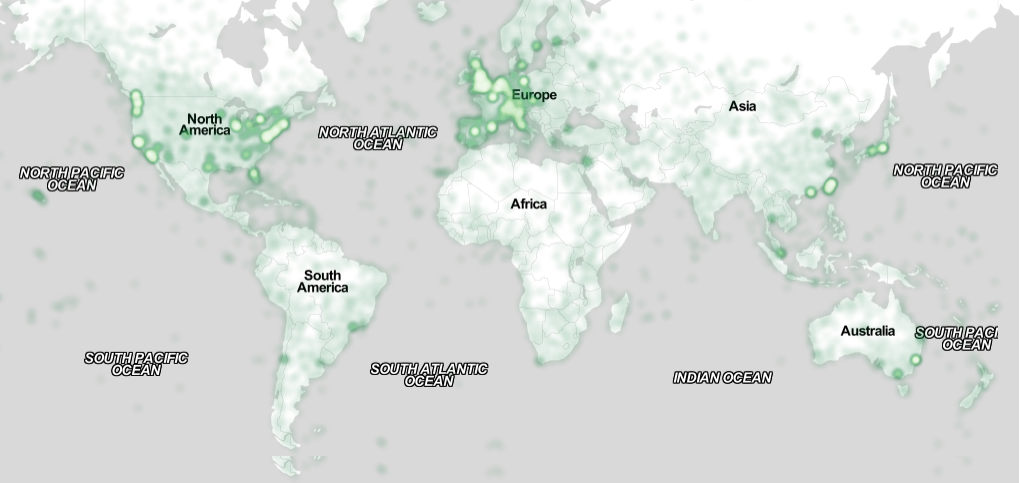
\includegraphics[width=0.9\columnwidth]{map.png}
\caption{A sample figure.}
\label{fig:map1}
\end{figure}

Figures spanning two columns can be set with the \texttt{figure*} environment as shown in figure~\ref{fig:map2}.

\begin{figure*}[tb]
\centering
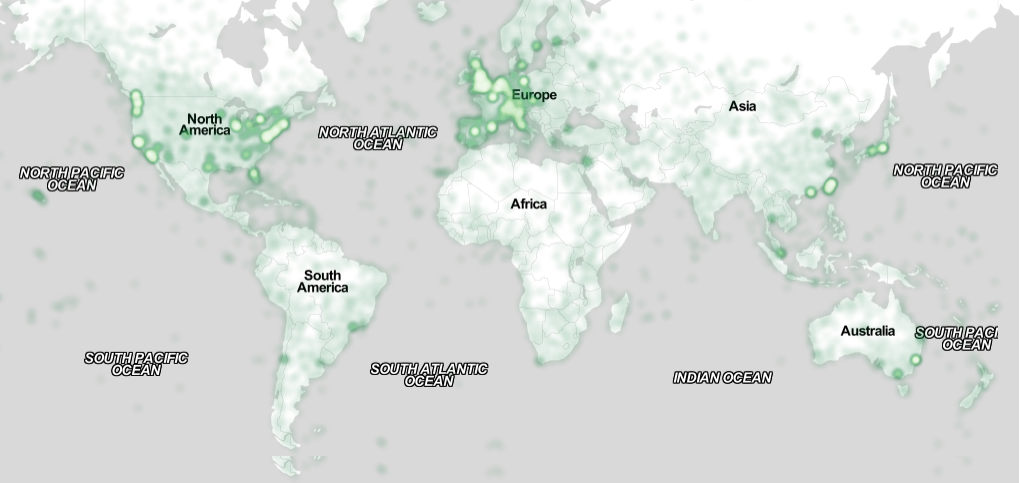
\includegraphics[width=0.9\textwidth]{map.png}
\caption{A sample figure spanning two columns.}
\label{fig:map2}
\end{figure*}


\section{Conclusions}
Some dummy texts to fill some space.

\subsection{Dutch}
Ik ben makelaar in koffi, en woon op de Lauriergracht No 37. Het is mijn gewoonte niet, romans te schrijven, of zulke dingen, en het heeft dan ook lang geduurd, voor ik er toe overging een paar riem papier extra te bestellen, en het werk aan te vangen, dat gij, lieve lezer, zoâven in de hand hebt genomen, en dat ge lezen moet als ge makelaar in koffie zijt, of als ge wat anders zijt. Niet alleen dat ik nooit iets schreef wat naar een roman geleek, maar ik houd er zelfs niet van, iets dergelijks te lezen, omdat ik een man van zaken ben.

Sedert jaren vraag ik mij af, waartoe zulke dingen dienen, en ik sta verbaasd over de onbeschaamdheid, waarmee een dichter of romanverteller u iets op de mouw durft spelden, dat nooit gebeurd is, en meestal niet gebeuren kan.Als ik in mijn vak -- ik ben makelaar in koffie, en woon op de Lauriergracht No 37 -- aan een principaal -- een principaal is iemand die koffie verkoopt -- een opgave deed, waarin maar een klein gedeelte der onwaarheden voorkwam, die in gedichten en romans de hoofdzaak uitmaken, zou hij terstond Busselinck \& Waterman nemen.

Dat zijn ook makelaars in koffie, doch hun adres behoeft ge niet te weten. Ik pas er dus wel op, dat ik geen romans schrijf, of andere valse opgaven doe. Ik heb dan ook altijd opgemerkt dat mensen die zich met zoiets inlaten, gewoonlijk slecht wegkomen. Ik ben drieënveertig jaar oud, bezoek sedert twintig jaren de beurs, en kan dus voor de dag treden, als men iemand roept die ondervinding heeft. Ik heb al wat huizen zien vallen! En gewoonlijk, wanneer ik de oorzaken naging, kwam het me voor, dat die moesten gezocht worden in de verkeerde richting die aan de meesten gegeven was in hun jeugd.

\subsection{Latin}
Lorem ipsum dolor sit amet, consectetur adipiscing elit. Nullam nec mi in neque rhoncus imperdiet et vel metus. Class aptent taciti sociosqu ad litora torquent per conubia nostra, per inceptos himenaeos. Morbi auctor vitae purus sit amet viverra. Nam facilisis urna id magna porttitor lobortis sed nec diam. Nullam sit amet laoreet lectus. Suspendisse convallis nulla ut finibus gravida. Nulla ut tortor eu tortor scelerisque accumsan non id leo. Interdum et malesuada fames ac ante ipsum primis in faucibus. Proin interdum, odio sit amet bibendum pretium, tortor ante aliquet libero, eget facilisis ligula diam finibus quam. Aenean auctor ornare neque, vel imperdiet lacus consequat ac. Mauris sed arcu nec sapien venenatis ullamcorper.

Duis elementum risus at eros vestibulum fringilla. Sed id felis quis arcu dignissim tincidunt et placerat est. Sed in finibus neque, a tristique felis. Aenean mollis ligula sed neque iaculis, id dignissim lorem vestibulum. Curabitur et purus at nulla eleifend facilisis in quis sem. Vivamus et justo vel risus dignissim maximus. Maecenas dapibus viverra felis eget interdum. Praesent venenatis sapien eu lectus porta fermentum. Aliquam nunc enim, sagittis id justo a, pellentesque sollicitudin magna. Etiam eget lacus dolor. Maecenas eget nisi ex. Nunc in pulvinar elit. Aenean efficitur velit nec egestas tincidunt.

Donec nec est egestas, pulvinar nibh et, sagittis arcu. Nullam in egestas elit. Praesent feugiat, lorem ac varius pharetra, nisl est efficitur odio, a elementum neque nibh nec lacus. Sed ac mauris ac massa vestibulum convallis in ac urna. Duis sed auctor eros, vel sodales est. Ut vulputate fermentum libero. Maecenas consectetur at dolor eu condimentum. Nam fringilla aliquam ipsum id scelerisque. Aenean vitae interdum urna. Aenean egestas ex sed euismod laoreet. Nulla sit amet velit felis. Maecenas a libero a dui mollis congue ut ac magna. Proin quis dictum velit. Praesent dapibus orci at nisi viverra hendrerit. Nam imperdiet blandit libero tempus bibendum.

\subsection{Kafka}
One morning, when Gregor Samsa woke from troubled dreams, he found himself transformed in his bed into a horrible vermin. He lay on his armour-like back, and if he lifted his head a little he could see his brown belly, slightly domed and divided by arches into stiff sections. The bedding was hardly able to cover it and seemed ready to slide off any moment.

His many legs, pitifully thin compared with the size of the rest of him, waved about helplessly as he looked. "What's happened to me? " he thought. It wasn't a dream. His room, a proper human room although a little too small, lay peacefully between its four familiar walls. A collection of textile samples lay spread out on the table - Samsa was a travelling salesman - and above it there hung a picture that he had recently cut out of an illustrated magazine and housed in a nice, gilded frame. It showed a lady fitted out with a fur hat and fur boa who sat upright, raising a heavy fur muff that covered the whole of her lower arm towards the viewer. Gregor then turned to look out the window at the dull weather. 


\appendix
%Appendix A
\section{Section in the Appendix}
Appendices can be used for additional material that do not fit into the main body in the paper but are still important. The main part should be understandable without the content in the appendices. Candidates for such content are lists of parameter settings, additional results (that show the same already shown before but on different data) or additional example images.

\begin{acks}
If you use special data sets or got some other help, here is the right place to mention it. Otherwise, this section can be left out.
\end{acks}


\bibliographystyle{ACM-Reference-Format}
\bibliography{sample-bibliography}

\end{document}
